\section{Geoprojected Ground Motion (GGM)}
\label{sec:ggm}

\subsection{Evaluation criteria}
\label{sec:ggm_criteria}

The evaluation of \acs{ggm} products is based on the relationship between the the input and output noise levels. The core idea is to evaluate how the spatial aggregation and inversion steps propagate or attenuate the noise present in the original \acs{gpro}/\acs{gpao} measurements. By estimating the expected noise in the output vectors as a function of the input noise characteristics and the resolution of the grid, the quality of the \acs{ggm} output can be quantitatively evaluated.

\subsection{Theoretical models}
\label{sec:ggm_models}
To retrieve the 3D surface displacement \(\mathbf{d} = [\textbf{d}^e, \textbf{d}^n, \textbf{d}^u]^\top\) (east, north, up), we consider four measurements:

\begin{itemize}
    \item \(\textbf{rg}_{\text{A}}\): range offset from ascending acquisition,
    \item \(\textbf{rg}_{\text{D}}\): range offset from descending acquisition,
    \item \(\textbf{az}_{\text{A}}\): azimuth offset from ascending acquisition,
    \item \(\textbf{az}_{\text{D}}\): azimuth offset from descending acquisition.
\end{itemize}

Each measurement can be expressed as a linear projection of the 3D displacement vector:

\[
\mathbf{d} = \mathbf{A} \mathbf{u}
\]

where \(\mathbf{d} \in \mathbb{R}^4\) is the measurement vector:

\[
\mathbf{d} =
\begin{bmatrix}
\textbf{rg}_{\text{A}} \\
\textbf{rg}_{\text{D}} \\
\textbf{az}_{\text{A}} \\
\textbf{az}_{\text{D}}
\end{bmatrix}
\]

and \(\mathbf{A} \in \mathcal{M}(4, 3, \mathbb{R})\) is the design matrix composed of the unit vectors projecting the 3D motion into each measurement geometry. For example:

\[
\mathbf{A} =
\begin{bmatrix}
\textbf{los}^{e}_{\text{A}} & \textbf{los}^{n}_{\text{A}} & \textbf{los}^{u}_{\text{A}} \\
\textbf{los}^{e}_{\text{D}} & \textbf{los}^{n}_{\text{D}} & \textbf{los}^{u}_{\text{D}} \\
\textbf{lof}^{e}_{\text{A}} & \textbf{lof}^{n}_{\text{A}} & \textbf{lof}^{u}_{\text{A}} \\
\textbf{lof}^{e}_{\text{D}} & \textbf{lof}^{n}_{\text{D}} & \textbf{lof}^{u}_{\text{D}} \\
\end{bmatrix}
\]

To estimate \(\mathbf{u}\), we solve the overdetermined system using the \acs{lmse} approach:

\[
\hat{\mathbf{u}} = (\mathbf{A}^\top \mathbf{A})^{-1} \mathbf{A}^\top \mathbf{d}
\]

\begin{figure}[h!]
\centering
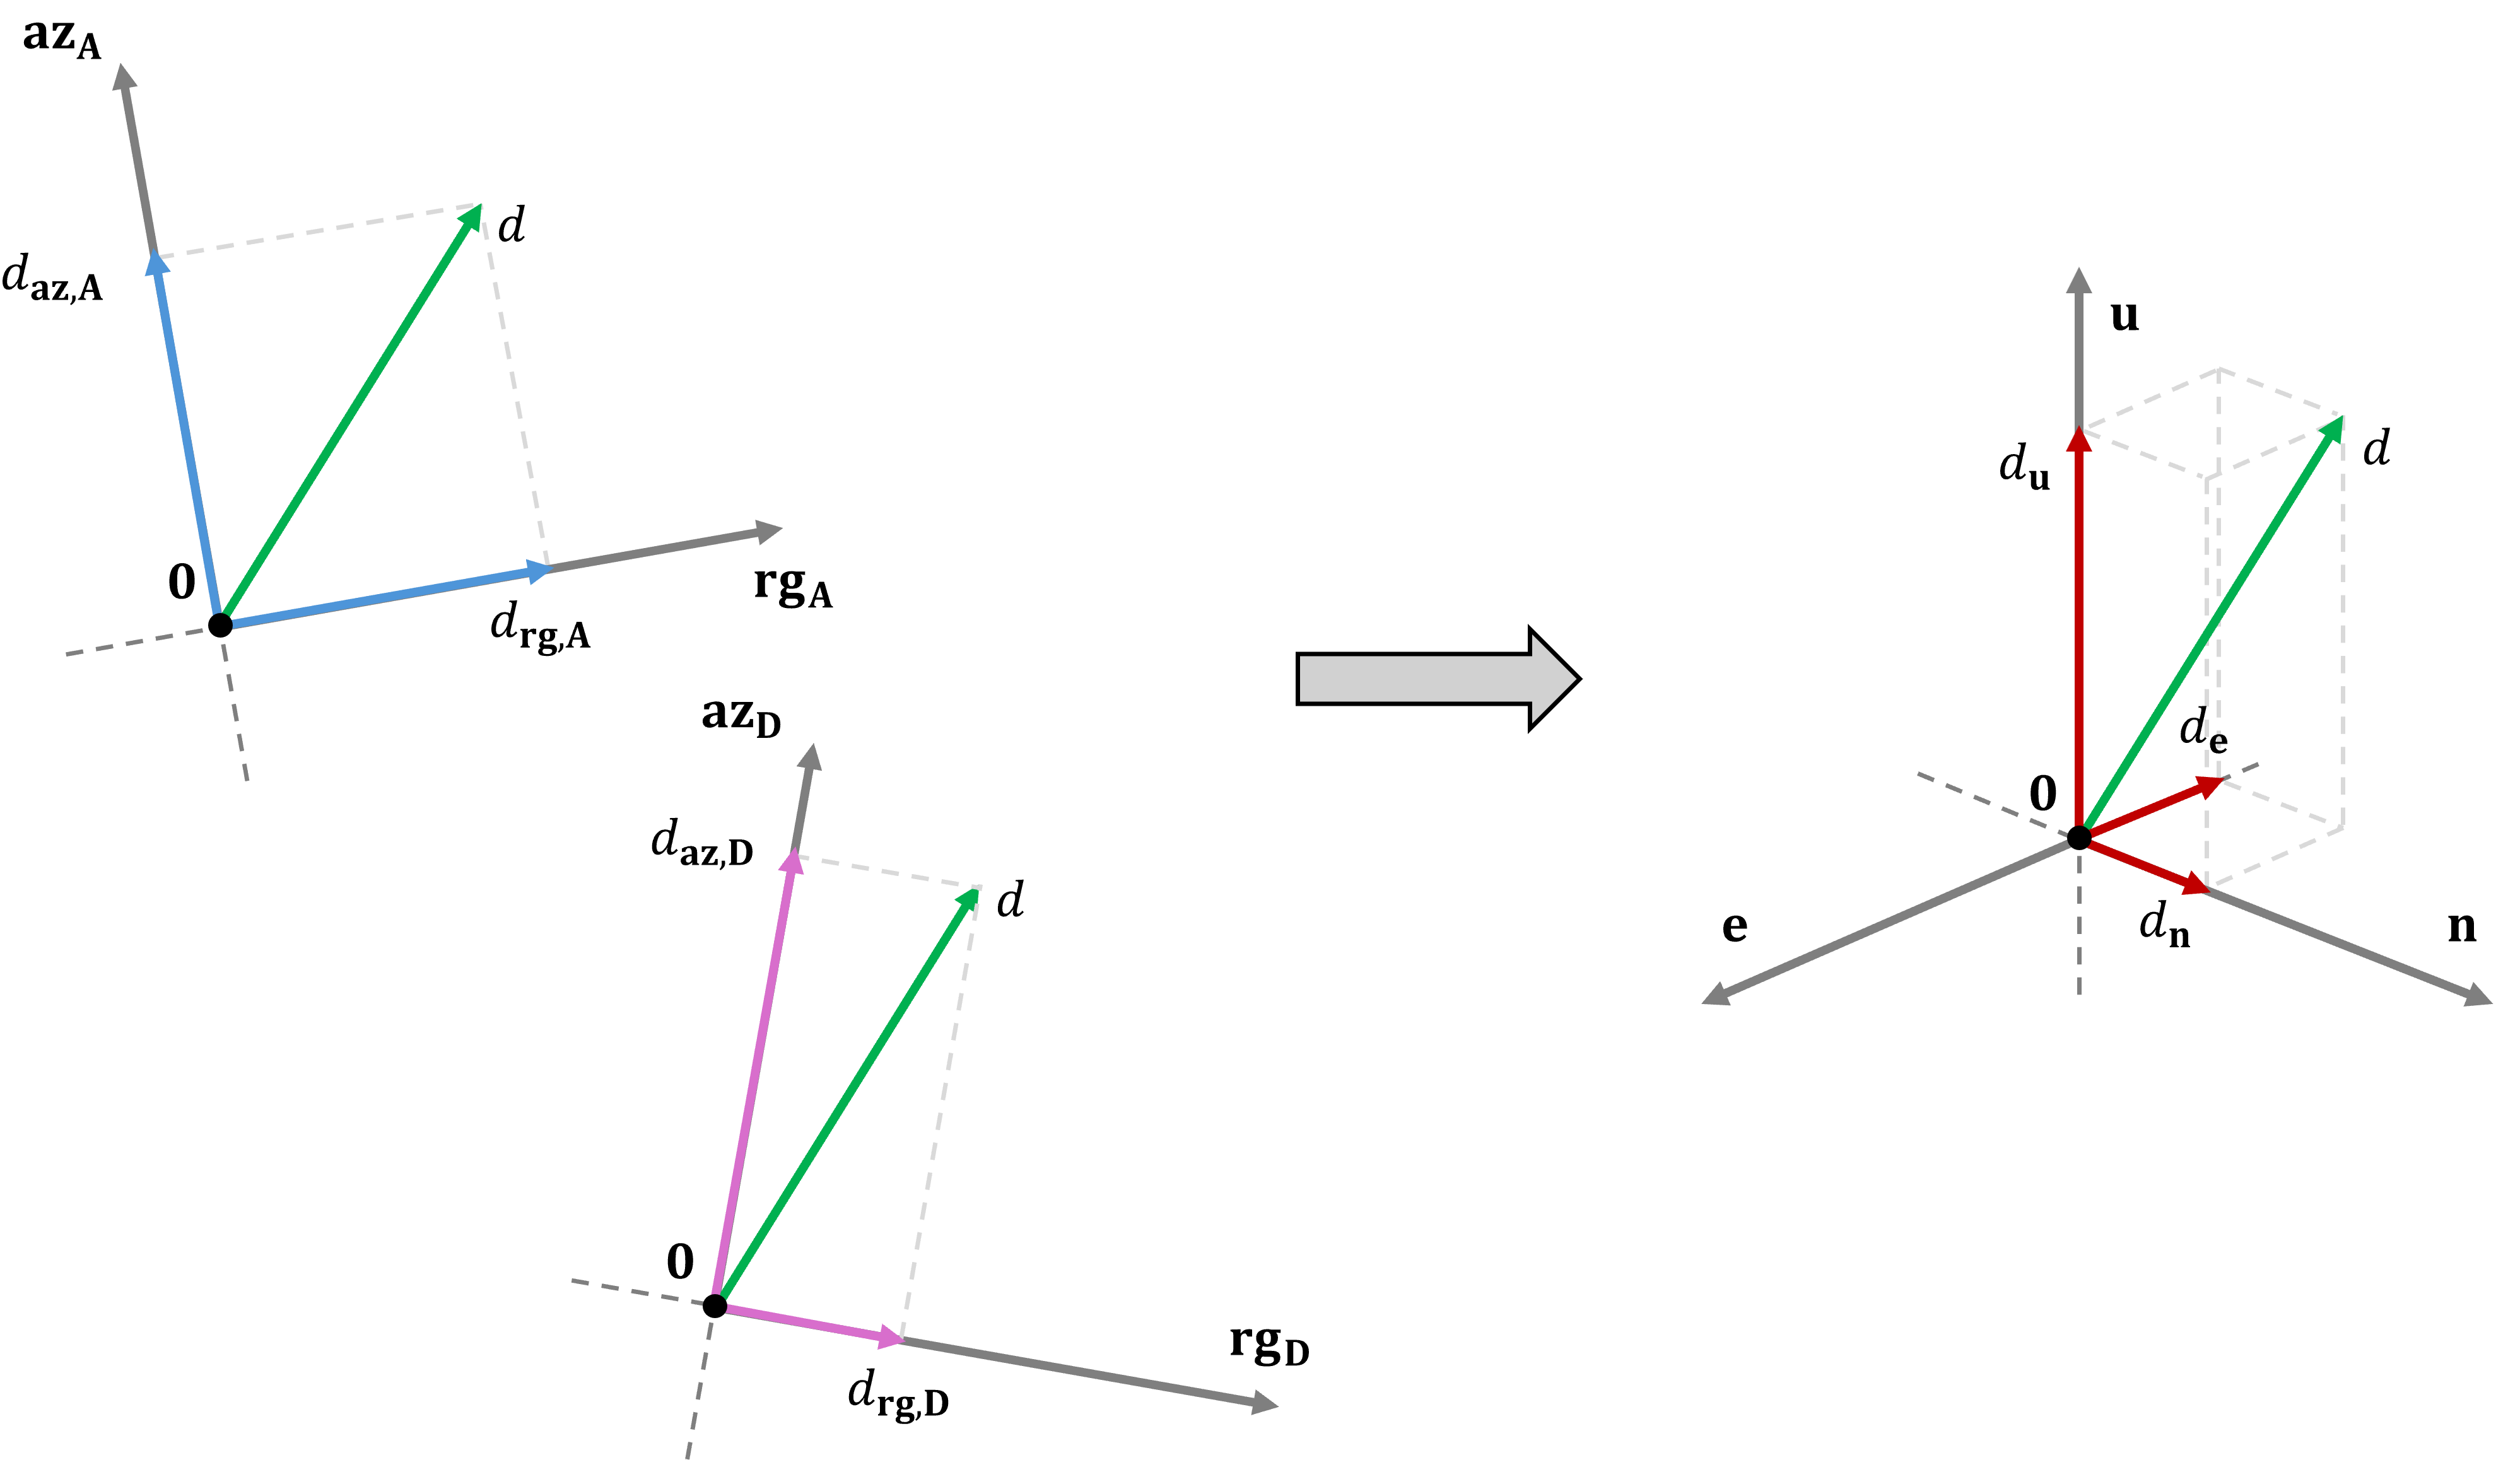
\includegraphics[width=15.0cm]{Figures/ggm/ggm_scheme.png}
\caption{Simple graphic scheme for the generation of the \acs{ggm} products starting from the \acs{pro}/\acs{pao} products.}
\end{figure}

If the measurement noise is not uniform, a weighted \acs{lmse} solution is more appropriate:

\[
\hat{\mathbf{u}} = (\mathbf{A}^\top \mathbf{W} \mathbf{A})^{-1} \mathbf{A}^\top \mathbf{W} \mathbf{d} = \mathbf{L} \mathbf{d}
\]

where \(\mathbf{W}\) is a diagonal weight matrix, typically set as the inverse variance of the measurements:

\[
\mathbf{W} = \operatorname{diag} \left( \sigma_{\text{A}, rg}^2, \sigma_{\text{D}, rg}^2, \sigma_{\text{A}, az}^2, \sigma_{\text{D}, az}^2 \right) ^ {-1}
\]

with \(\sigma_r\) and \(\sigma_a\) representing the standard deviations of range and azimuth offsets, respectively, and \( \mathbf{L} = (\mathbf{A}^\top \mathbf{W} \mathbf{A})^{-1} \mathbf{A}^\top \mathbf{W} \).

Given the significantly different noise levels associated with azimuth and range offsets in \acs{s1} and \acs{rosel} data, it is critical to account for these discrepancies when assessing or improving the accuracy of derived ground motion products: the azimuth offset accuracy is indeed one or two orders of magnitude worse than the range offset accuracy. To mitigate the high noise in azimuth offsets and enhance the reliability of azimuth-constrained products, it is advisable to spatially coarsen the azimuth resolution (for instance, through multilook). This spatial aggregation can reduce the effective noise level, depending on the size of the averaging window. 

\subsection{Computational complexity}
\label{sec:ggm_computation}

The generation of \acs{ggm} products from \acs{gpro}/\acs{gpao} input products follows a three-steps process:

\begin{itemize}
    \item \acs{gpao} products typically exhibit significantly lower resolution in the azimuth direction compared to GPRO products. To mitigate this and ensure more balanced noise characteristics, a uniform filter is applied to GPAO measurements. This filtering step ensures that the resulting noise levels become comparable to those of full-resolution \acs{gpro} data.

    \item The geographical coverage of the input \acs{gpro}/\acs{gpao} products is analyzed to determine their spatial extent. A regular metric grid is then defined to cover the intersection area of the inputs. The resolution of this grid is chosen based on the desired spatial granularity and serves as an implicit estimate of the input (and consequently output) noise level. Within each grid cell, all input data points that fall inside the cell are aggregated, typically through an arithmetic averaging process. This spatial averaging helps to reduce noise and prepare the data for the inversion step. The corresponding \acs{los}/\acs{lof} vectors are averaged in the same way.

    \item For each populated grid cell, a linear system of equations of size \( 4 \times 3 \) is constructed using the averaged input data. This system is then solved using a linear \acs{lmse} approach to estimate the 3-dimensional output vector (North-South, East-West, Vertical) for each cell. This inversion is performed independently for each grid cell. Further details are provided in \ref{sec:ggm_models}.
\end{itemize}

Let \( M \) and \( N \) denote, respectively, the maximum acquisition length (in azimuth pixels) and the maximum swath width (in range pixels) for all input products (without loss of generality, we assume that for each input product, the azimuth dimension is at most \( M \) pixels and the range dimension is at most \( N \) pixels).

The complexity of the preprocessing step is linear in the number of input pixels (\( \mathcal{O}(M \times N) \)), since the uniform filter is applied with constant cost per pixel.

The number of output grid cells, denoted \( N_C \), is also proportional to \( M \times N \). Both the averaging step and the linear inversion step are applied once per output cell: since the inversion involves solving a fixed-size (\( 4 \times 3 \)) linear system and the number of input measurements per cell is limited by the grid resolution, the per-cell cost is constant. Therefore, the complexity of both steps is also \( \mathcal{O}(N_C) = \mathcal{O}(M \times N) \).

In conclusion, the total computational complexity of the entire process is linear in the number of input image pixels:
\[
C_{\text{tot}} = \mathcal{O}(M \times N)
\]

\subsection{Criticalities and weakness}
\label{sec:ggm_criticalities}

The \acs{ggm} products inherit all the intrinsic limitations and potential inaccuracies of their input data, the \acs{gpro} and \acs{gpao} products. Any systematic errors, noise characteristics, or biases present in the input measurements or their respective processing pipelines will propagate into the final \acs{ggm} outputs.

An additional critical aspect arises from the anisotropic resolution of the input data, particularly in the case of \acs{gpao} products: these products typically exhibit significantly heigher noise with respect to \acs{gpro} products. If left unaddressed, this anisotropy can lead to numerical instability or ill-posedness in the per-cell linear inversion step, as the underlying linear systems may become sensitive to directional noise and lack robustness. To mitigate this issue, a uniform spatial filtering operation is applied as a preprocessing step to \acs{gpao} measurements. This step is crucial to homogenize the noise characteristics across all input products, thereby improving the conditioning of the inversion systems. However, this comes at the cost of reduced spatial resolution for \acs{gpao} products, and may result in some loss of local detail in the final \acs{ggm} output.

In summary, while the preprocessing step is essential to ensure numerical stability and consistent noise behavior in the inversion process, it also represents a trade-off between robustness and spatial fidelity. These factors, together with inherited input limitations, must be carefully considered when interpreting or applying \acs{ggm} products.

